
\documentclass[xcolor=dvipsnames, xcolor=table]{beamer} % Classe de documento para apresentações

\usepackage{listings}\usetheme{Berlin}
\usecolortheme{beaver}
\usepackage{textpos}
\usepackage{color}
\usepackage{wasysym}
\renewcommand\tabcolsep{4pt}
\usepackage{csquotes} 
\usepackage{wrapfig}
\usepackage{microtype}
\usepackage[labelfont=bf]{caption}
\usepackage{epigraph}
\usepackage[english]{babel}
\usepackage{float}
\usepackage{hyperref}
%\hypersetup{colorlinks=true,linkcolor=blue}
\usepackage{amsmath}
\newcommand{\dd}[1]{\mathrm{d}#1}
\usepackage{amsfonts}
\usepackage{amssymb}
\usepackage{amsbsy}
\usepackage{graphicx}
\usepackage{mathtools}

\usepackage{booktabs}

\usepackage{adjustbox}
\hypersetup{pdfpagemode=FullScreen} % para o pdf abrir automaticamente em modo full screen
\setbeamertemplate{caption}[numbered] % para numerar as tabelas
\usepackage{subcaption}
\usepackage[none]{hyphenat} 
\usepackage{bm} %%% bold vectors
\usepackage{tabularx}  
\usepackage{tikz}

\setbeamercolor{author in head/foot}{fg=Maroon}     % cor do nome do autor no rodape
\setbeamercolor{institute in head/foot}{fg=Maroon}  % cor do nome do ISEG no rodape
\setbeamercolor{frametitle}{fg=Maroon, bg=black!9} % cor da letra e do fundo fa faixa com o nome de cada slide
\setbeamercolor{caption name}{fg=Maroon, bg=black!9}
\setbeamercolor*{title}{fg=white, bg=Maroon}          % cor do titulo e da caixa de titulo na capa
\setbeamercolor{itemlist item}{fg=Maroon}               % cor dos bullets do ambiente \itemlist 

\setbeamertemplate{section in toc}[circle]
\setbeamercolor{section number projected}{bg=Maroon,fg=white}
\setbeamercolor{subsection number projected}{bg=Maroon,fg=white}

\setbeamercolor{block title}{fg=Maroon} % color of enumerated items
\setbeamercolor{local structure}{fg=Maroon} % color of enumerated items


\makeatletter % criaçao de um ambiente sem TOC no cabeçalho do slide
\newenvironment{noheadline}{
\setbeamertemplate{headline}{}
\addtobeamertemplate{frametitle}{\vspace*{-0.9\baselineskip}}{}
}{}
\makeatother

\usepackage[beamer,customcolors]{hf-tikz}

\tikzset{hl/.style={
    set fill color=red!80!black!40,
    set border color=red!80!black,
  },
}


\title[Getting Started]{Getting Started}
\author[João Vieira \& Pedro Fonseca]{\textbf {João Vieira \& Pedro Fonseca}}
\titlegraphic{
\includegraphics[width=1.5cm]{yes}}
\institute[Introduction to R Programming]{\textbf {Introduction to R Programming}}
\date{\today}


% position the yes
\addtobeamertemplate{frametitle}{}{%
\begin{textblock*}{100mm}(.85\textwidth,-.9cm)

\includegraphics[scale=.05]{yes}
\end{textblock*}}



%%%%%%%%%%%%% Ambiente de teorema/definição com as cores do ISEG %%%%%%

\makeatletter
\def\th@mystyle{%
    \normalfont % body font
    \setbeamercolor{block title example}{bg=Maroon,fg=white}
    \setbeamercolor{block body example}{bg=black!9,fg=black}
    \def\inserttheoremblockenv{exampleblock}
  }
\makeatother
\theoremstyle{mystyle}
\newtheorem*{defi}{Definição}

\setbeamertemplate{defis}[numbered]



%%%%%%%%%%%%%%%% Bibliografia %%%%%%%%%%%%%%%%%%%%%%%

\usepackage{url}
\usepackage[style=authoryear, bibencoding=utf8, minnames=1, maxnames=3,
maxbibnames=99,backref=true, natbib=true, dashed=false, terseinits=true, 
firstinits=true, uniquename=false, uniquelist=true, labeldate=true, 
doi=false, isbn=false, natbib=true, backend=biber]{biblatex}
\DefineBibliographyStrings{english}{%
    backrefpage = {Cited on page},
    backrefpages = {Cited on pages},
}
% Change the default formatting to be more "statistical"
\DeclareFieldFormat{url}{\url{#1}}
\DeclareFieldFormat[article]{pages}{#1}
\DeclareFieldFormat[inproceedings]{pages}{\lowercase{pp.}#1}
\DeclareFieldFormat[incollection]{pages}{\lowercase{pp.}#1}
\DeclareFieldFormat[article]{volume}{\mkbibbold{#1}}
\DeclareFieldFormat[article]{number}{\mkbibparens{#1}}
\DeclareFieldFormat[article]{title}{\MakeCapital{#1}}
\DeclareFieldFormat[article]{url}{}
\DeclareFieldFormat[book]{url}{}
\DeclareFieldFormat[inbook]{url}{}
\DeclareFieldFormat[incollection]{url}{}
\DeclareFieldFormat[inproceedings]{url}{}
\DeclareFieldFormat[inproceedings]{title}{#1}
\DeclareFieldFormat{shorthandwidth}{#1}
% No dot before number of articles
\usepackage{xpatch}
\xpatchbibmacro{volume+number+eid}{\setunit*{\adddot}}{}{}{}
% Remove In: for an article.
\renewbibmacro{in:}{%
  \ifentrytype{article}{}{%
  \printtext{\bibstring{in}\intitlepunct}}}
% Get rid of months in citations
\AtEveryBibitem{\clearfield{month}}
\AtEveryCitekey{\clearfield{month}}
\setlength{\parindent}{1,3cm}
\raggedbottom

\renewcommand\bibfont{\scriptsize}
% If you have more than one page of references, you want to tell beamer
% to put the continuation section label from the second slide onwards
\setbeamertemplate{frametitle continuation}[from second]
% Now get rid of all the colours
\setbeamercolor*{bibliography entry title}{fg=black}
\setbeamercolor*{bibliography entry author}{fg=black}
\setbeamercolor*{bibliography entry location}{fg=black}
\setbeamercolor*{bibliography entry note}{fg=black}



\begin{document}
%%%%%%%%%%%%%%%%%%%%%  CAPA  %%%%%%%%%%%%%%%%%%%%%%%%%%%%%
\begin{noheadline}

\begin{frame}%[plain]
\vfill
\centering

\begin{beamercolorbox}[sep=8pt,center,colsep=-4bp,rounded=true,shadow=true]{title}
\usebeamerfont{title}\inserttitle\par%
\ifx\insertsubtitle\@empty%
\else%
\vskip0.25em%
{\usebeamerfont{subtitle}\usebeamercolor[fg]{subtitle}\insertsubtitle\par}%
\fi%     
\end{beamercolorbox}%

\vskip1em\par

\begin{beamercolorbox}[sep=8pt,center,colsep=-4bp,rounded=true,shadow=true]{author}
\usebeamerfont{author}\insertauthor
\end{beamercolorbox}

{\usebeamercolor[fg]{titlegraphic}\inserttitlegraphic\par}

\begin{beamercolorbox}[sep=8pt,center,colsep=-4bp,rounded=true,shadow=true]{institute}
\usebeamerfont{institute}\insertinstitute
\end{beamercolorbox}

\begin{beamercolorbox}[sep=8pt,center,colsep=-4bp,rounded=true,shadow=true]{date}
\usebeamerfont{date}\insertdate
\end{beamercolorbox}\vskip0.5em

\end{frame}
\end{noheadline}



%%%%%%%%%%%%%% itemlist SHAPES AND COLLERS%%%%%%%%%%%%%%%%%%%%%%%%%

\setbeamertemplate{itemize item}{\color{Maroon}\newmoon}
\setbeamertemplate{itemize subitem}{\color{Maroon}$\blacktriangleright$}

%%%%%%%%% TABLE OF CONTENTS SHAPES, COLLORS AND BULLETS %%%%%%%%%%%%%%%%


%%%%%%%%%%%%%%%%%%%%%%%%%%%%%%%%%%%%%%%%%%%%%%%%%%%%%%%%%%%%%%%

\begin{noheadline}

\begin{frame}[allowframebreaks]
	\frametitle{Contents}
    \tableofcontents[hideallsubsections]
\end{frame}

\end{noheadline}

%%%%%%%%%%%%%%%%%%%%%%%%%%%%%%%%%%%%%%%%%%%%%%%%%%%%%%%%%%%%%%%


%%%%%%%%%%%%%%%%%%%%%%%%%%%%%%%%%%%%%%%%%%%%%%%%%%%%%%%%%%%%%%%

\section{R and Rstudio} 

\subsection{What is R?}

\begin{frame}[fragile] %%%%%%%%%%%%%%%%%%%%%%% FRAME %%%%%%%%%%%%%%%%%%%%%%%%%%%%
\frametitle{R vs Rstudio}

\begin{itemize}

\item R is a programming language and free software environment for statistical computing and graphics.	
\item RStudio is an integrated development environment (IDE) for R.
\item R and Rstudio are not two different versions of the same thing. 
\item You can use R without using RStudio, but you can't use Rstudio without using R.

\end{itemize}
	
\end{frame}

\begin{frame} %%%%%%%%%%%%%%%%%%%%%%% FRAME %%%%%%%%%%%%%%%

\frametitle{This is How R Looks Like}

\begin{figure}[H]
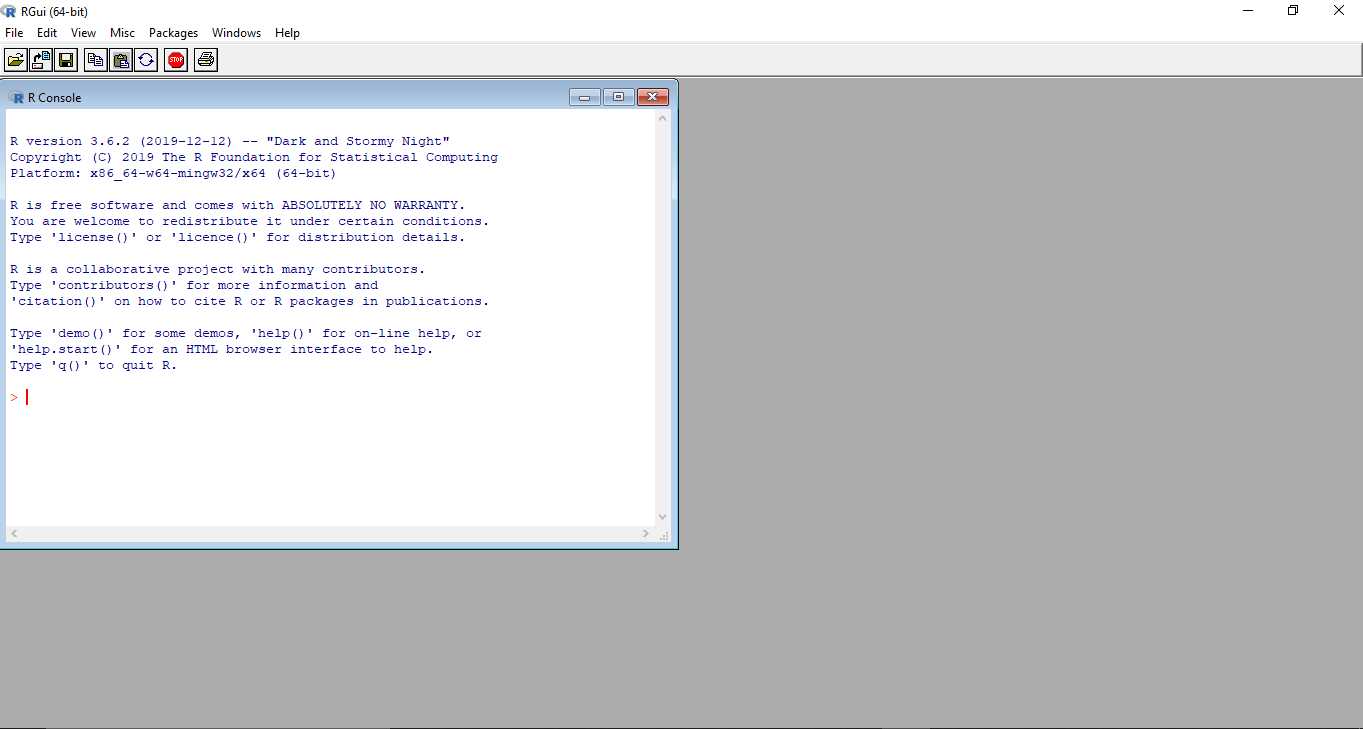
\includegraphics[scale = .28]{Screenshot_1}
\caption{R console on windows}
\end{figure}

\end{frame}

\begin{frame} %%%%%%%%%%%%%%%%%%%%%%% FRAME %%%%%%%%%%%%%%%

\frametitle{This is How R Looks Like}

\begin{figure}[H]
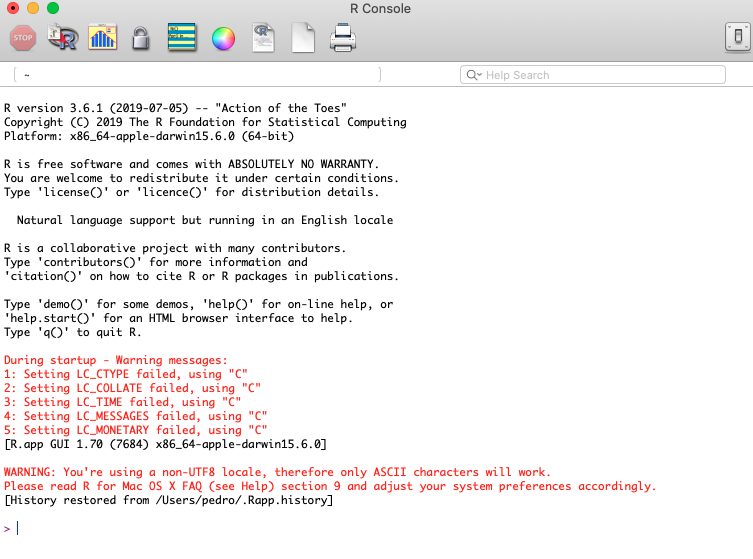
\includegraphics[scale = .27]{r-mac}
\caption{R console on MacOS}
\end{figure}

\end{frame}

\begin{frame} %%%%%%%%%%%%%%%%%%%%%%% FRAME %%%%%%%%%%%%%%%
\frametitle{This is How R Looks Like}

\begin{figure}[H]
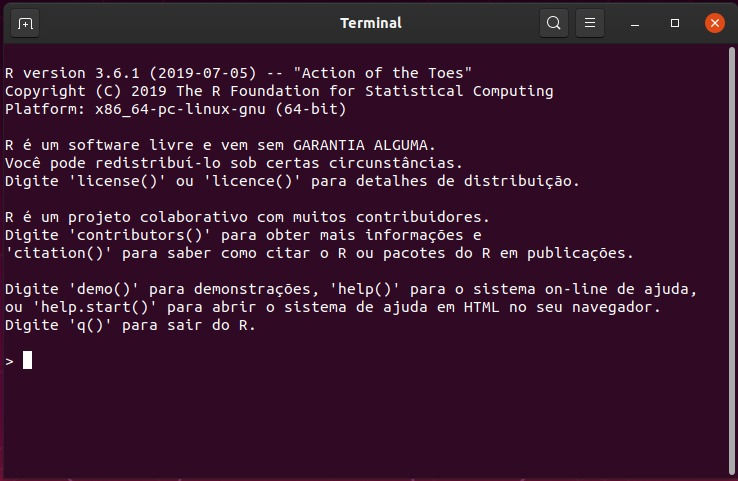
\includegraphics[scale = .3]{r-linux}
\caption{R console on Linux}
\end{figure}

\end{frame}

\begin{frame} %%%%%%%%%%%%%%%%%%%%%%% FRAME %%%%%%%%%%%%%%%
\frametitle{This is How Rstudio Looks Like}
\begin{figure}[H]
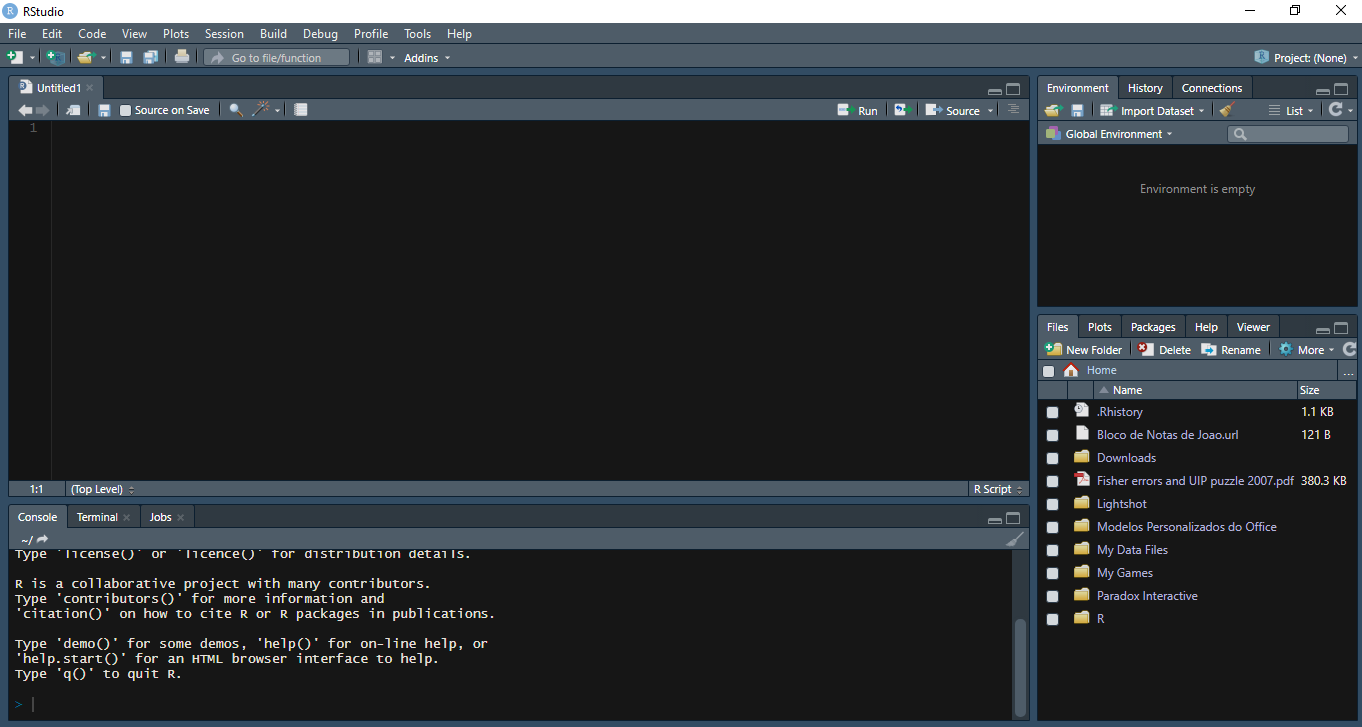
\includegraphics[scale = 0.28]{Screenshot_2}%
\caption{Rstudio on Windows and Linux}
\end{figure}

\end{frame}

\begin{frame} %%%%%%%%%%%%%%%%%%%%%%% FRAME %%%%%%%%%%%%%%%

\begin{figure}[H]
\frametitle{This is How Rstudio Looks Like}

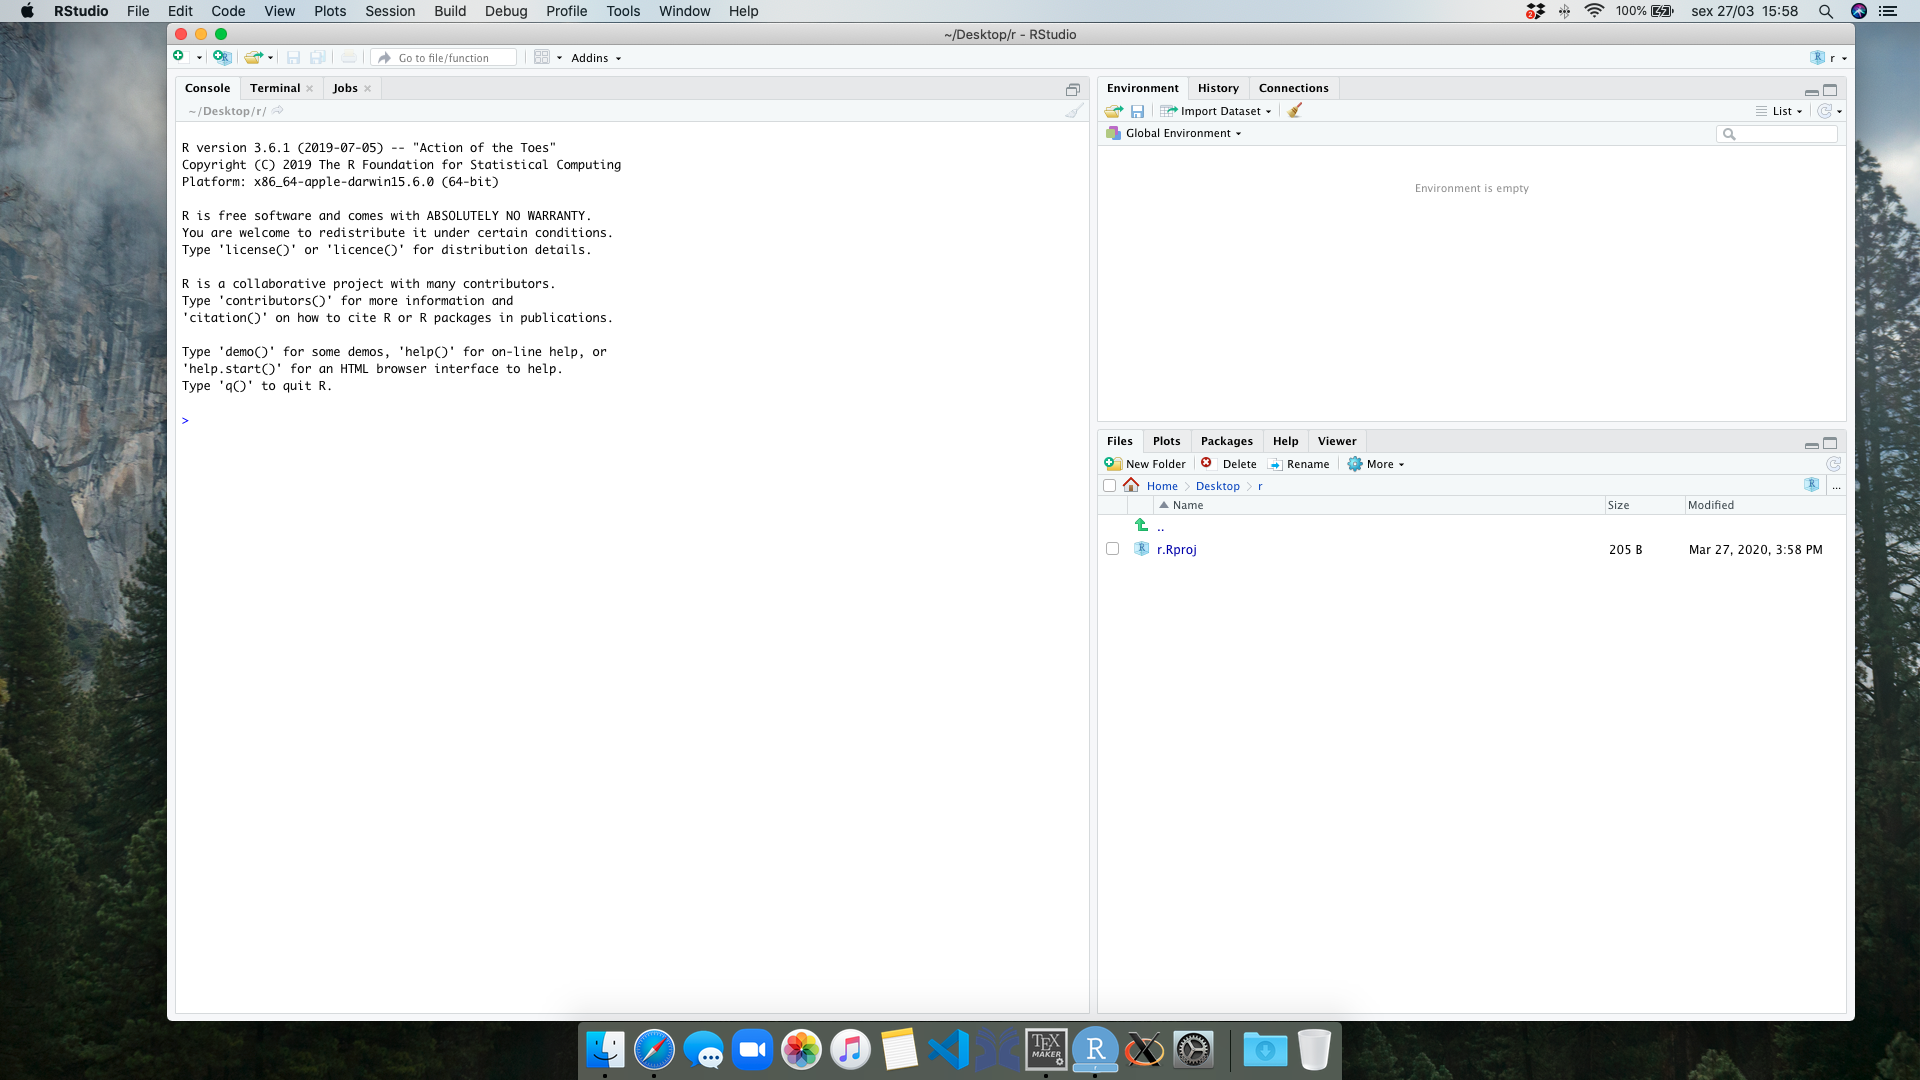
\includegraphics[scale = 0.14]{Screenshot_mac}%
\caption{Rstudio on MacOS}

\end{figure}

\end{frame}


\begin{frame}[fragile] %%%%%%%%%%%%%%%%%%%%%%% FRAME %%%%%%%
\frametitle{Rstudio Cloud}
\begin{itemize}

\item If you don't want to install R and RStudio:		

\begin{enumerate}

\item Go to \href{https://rstudio.cloud/}{\textcolor{blue}{RStudio Cloud}}.

\item Create an account and login.

\item Click "New Project".

\end{enumerate}	

\end{itemize}

\end{frame}


\begin{frame}[fragile] %%%%%%%%%%%%%%%%%%%%%%% FRAME %%%%%
\frametitle{Rstudio Cloud}
\begin{itemize}
\item You should then see something like this:
\end{itemize}

\begin{figure}[H]
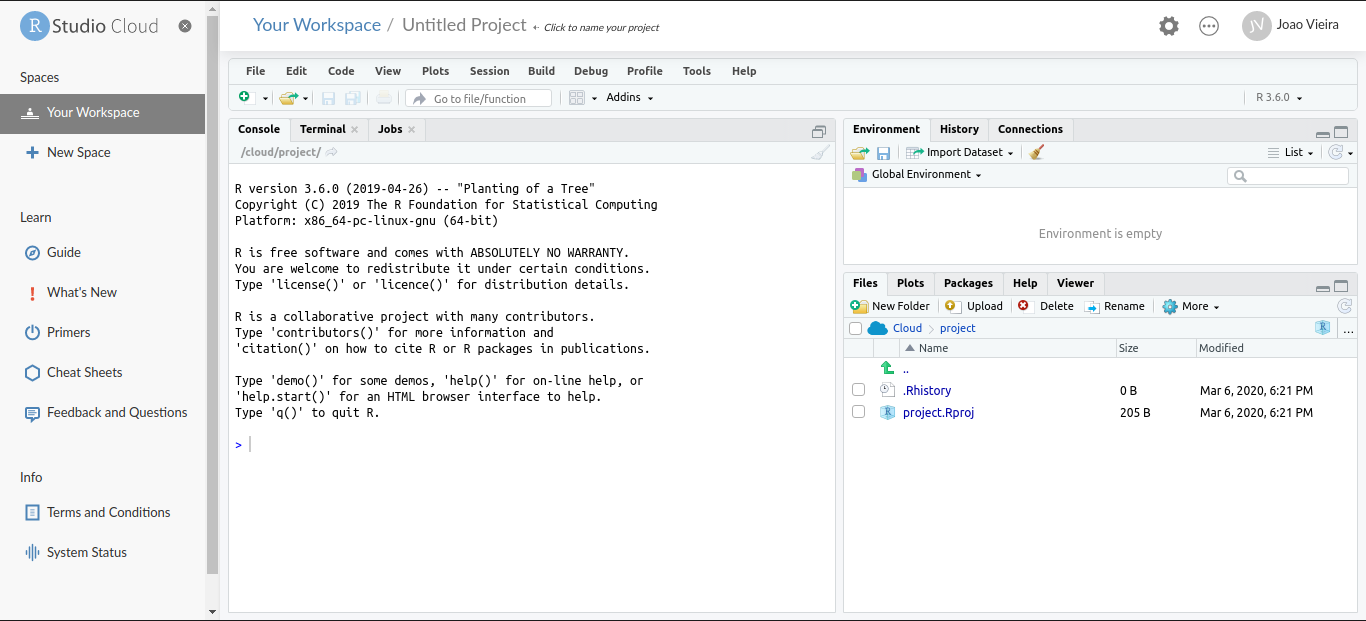
\includegraphics[scale = .2]{Screenshot_6} 
\caption{Rstudio Cloud}
\end{figure}

\begin{itemize}
\item For additional information: \href{https://rstudio.cloud/learn/guide}{\textcolor{blue}{https://rstudio.cloud/learn/guide}}
\end{itemize}
	
\end{frame}

\section{Workflow}
\subsection{Rstudio Projects}

\begin{frame}
\frametitle{Your First Project}
\begin{figure}
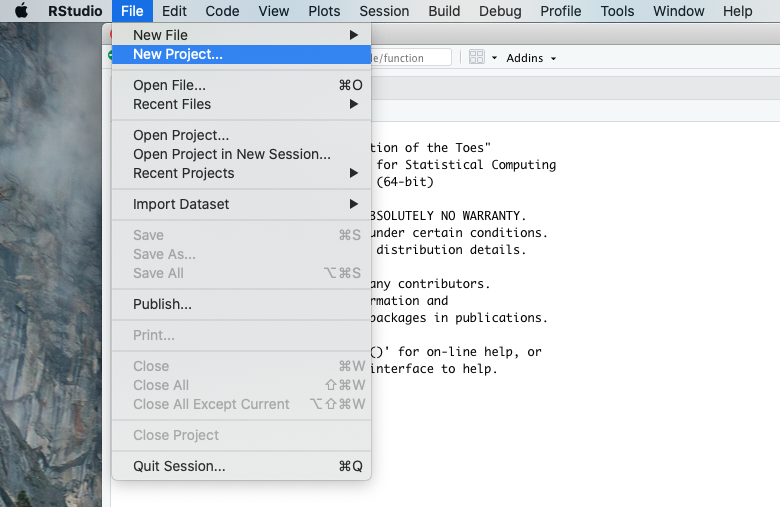
\includegraphics[scale=0.3]{new-project-1.png}
\end{figure}
\end{frame}

\begin{frame}
\frametitle{Your First Project}
\begin{figure}
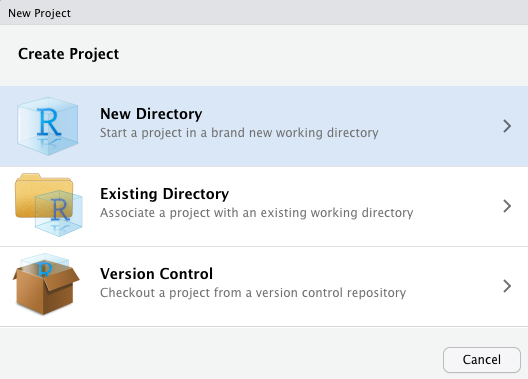
\includegraphics[scale=0.4]{new-project-2.png}
\end{figure}
\end{frame}

\begin{frame}
\frametitle{Your First Project}
\begin{figure}
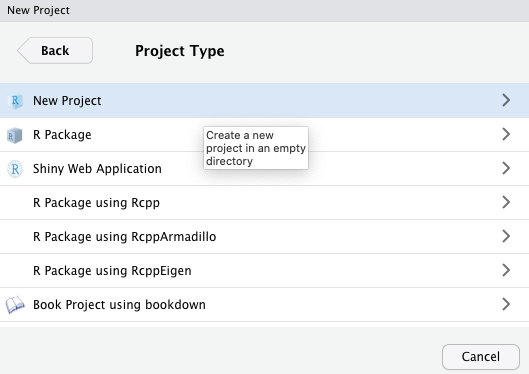
\includegraphics[scale=0.4]{new-project-3.png}
\end{figure}
\end{frame}

\begin{frame}
\frametitle{Your First Project}
\begin{figure}
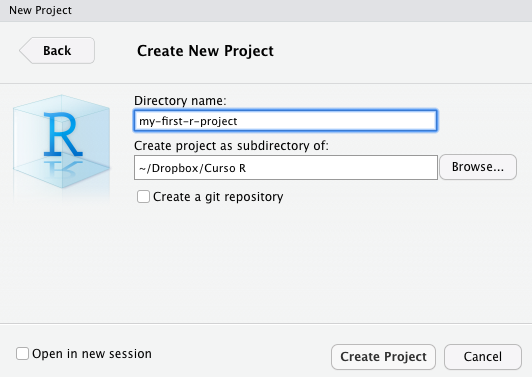
\includegraphics[scale=0.4]{new-project-4.png}
\end{figure}
\end{frame}

\begin{frame}
\frametitle{Your First Project}
\begin{figure}
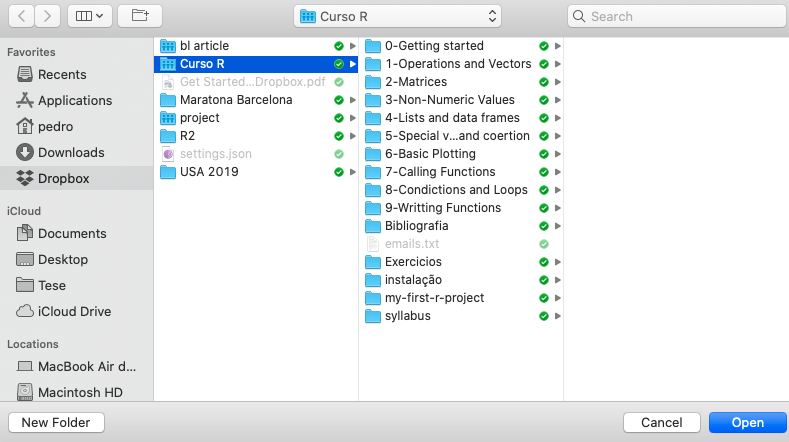
\includegraphics[scale=0.3]{new-project-5.png}
\end{figure}
\end{frame}

\begin{frame}
\frametitle{Your First Project}
\begin{figure}
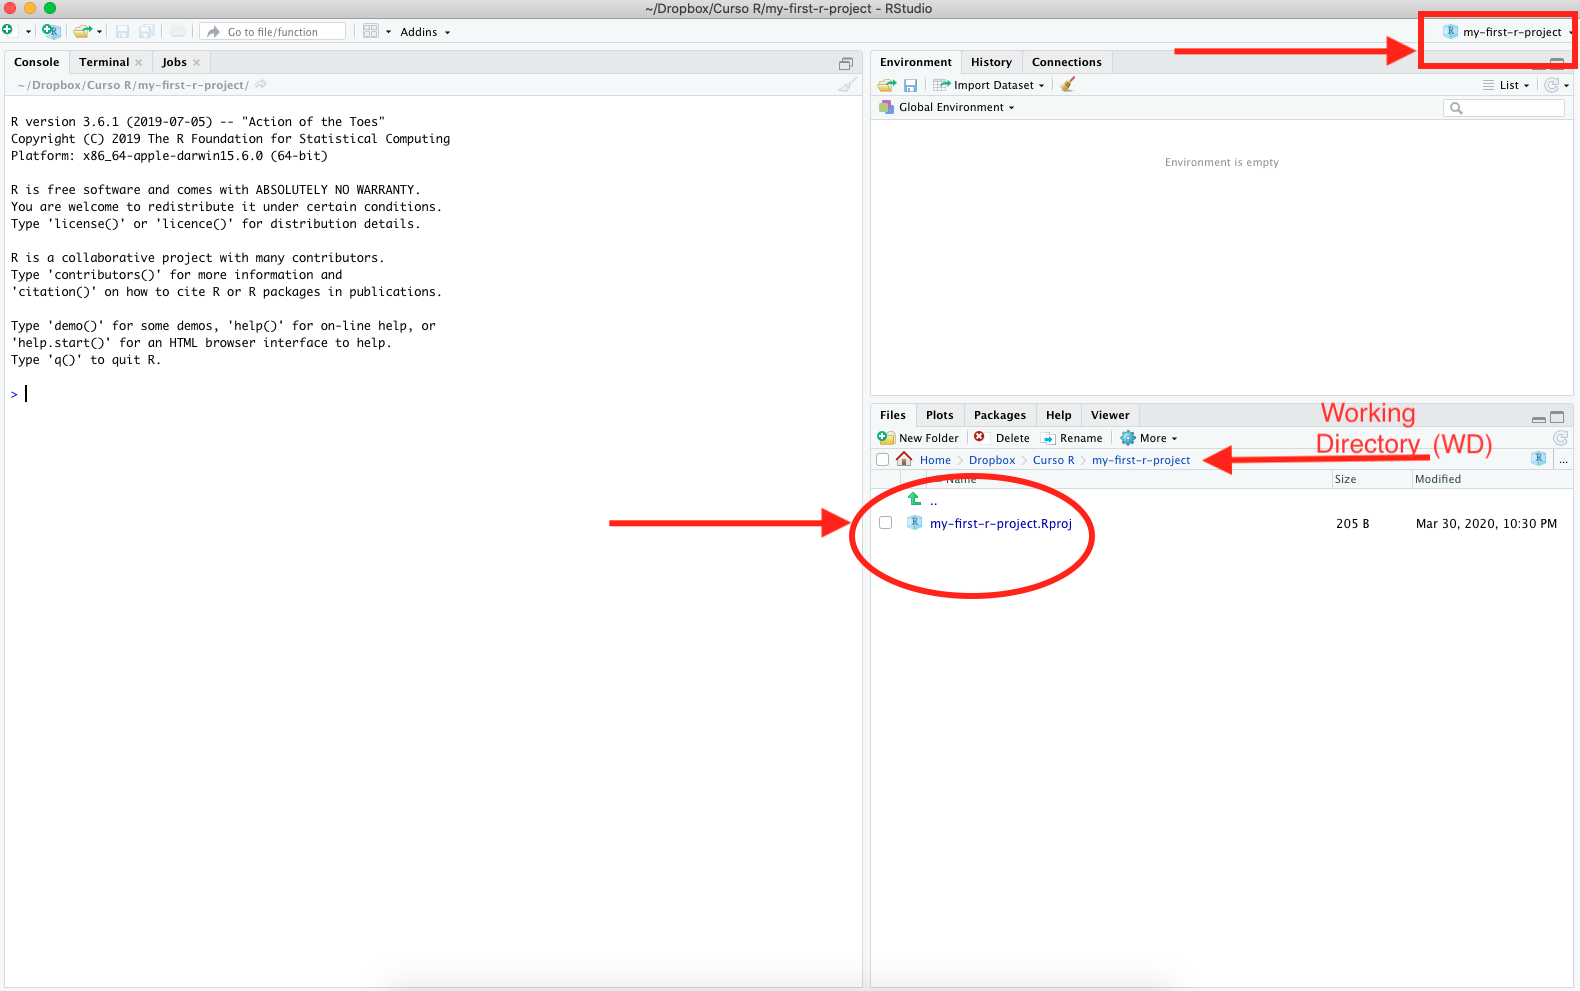
\includegraphics[scale=0.16]{environment.png}
\end{figure}
\end{frame}

\subsection{Scripts, Console and Environment}

\begin{frame}
\frametitle{Your First R Script}
\begin{figure}
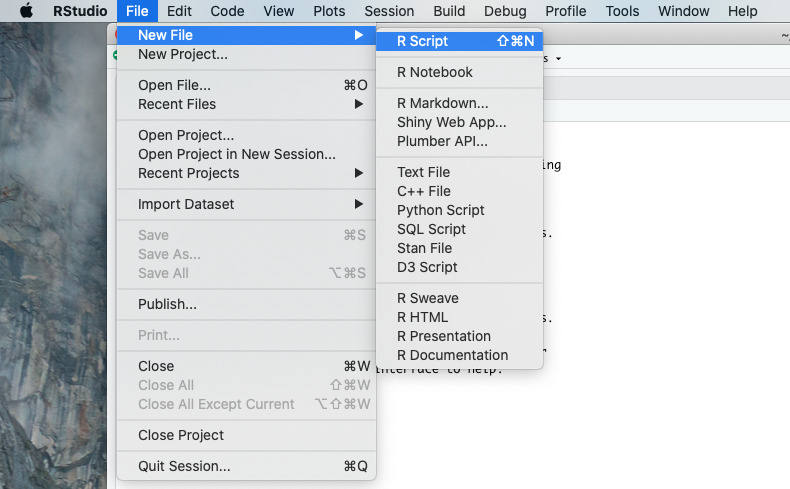
\includegraphics[scale=0.29]{new-script.png}
\end{figure}

\begin{itemize}
\item Shortcut: Cmd+Shift+N (Mac) or Ctrl+Shift+N (Windows and Linux)
\end{itemize}
\end{frame}

\begin{frame}
\frametitle{Rstudio Panes}
\begin{figure}
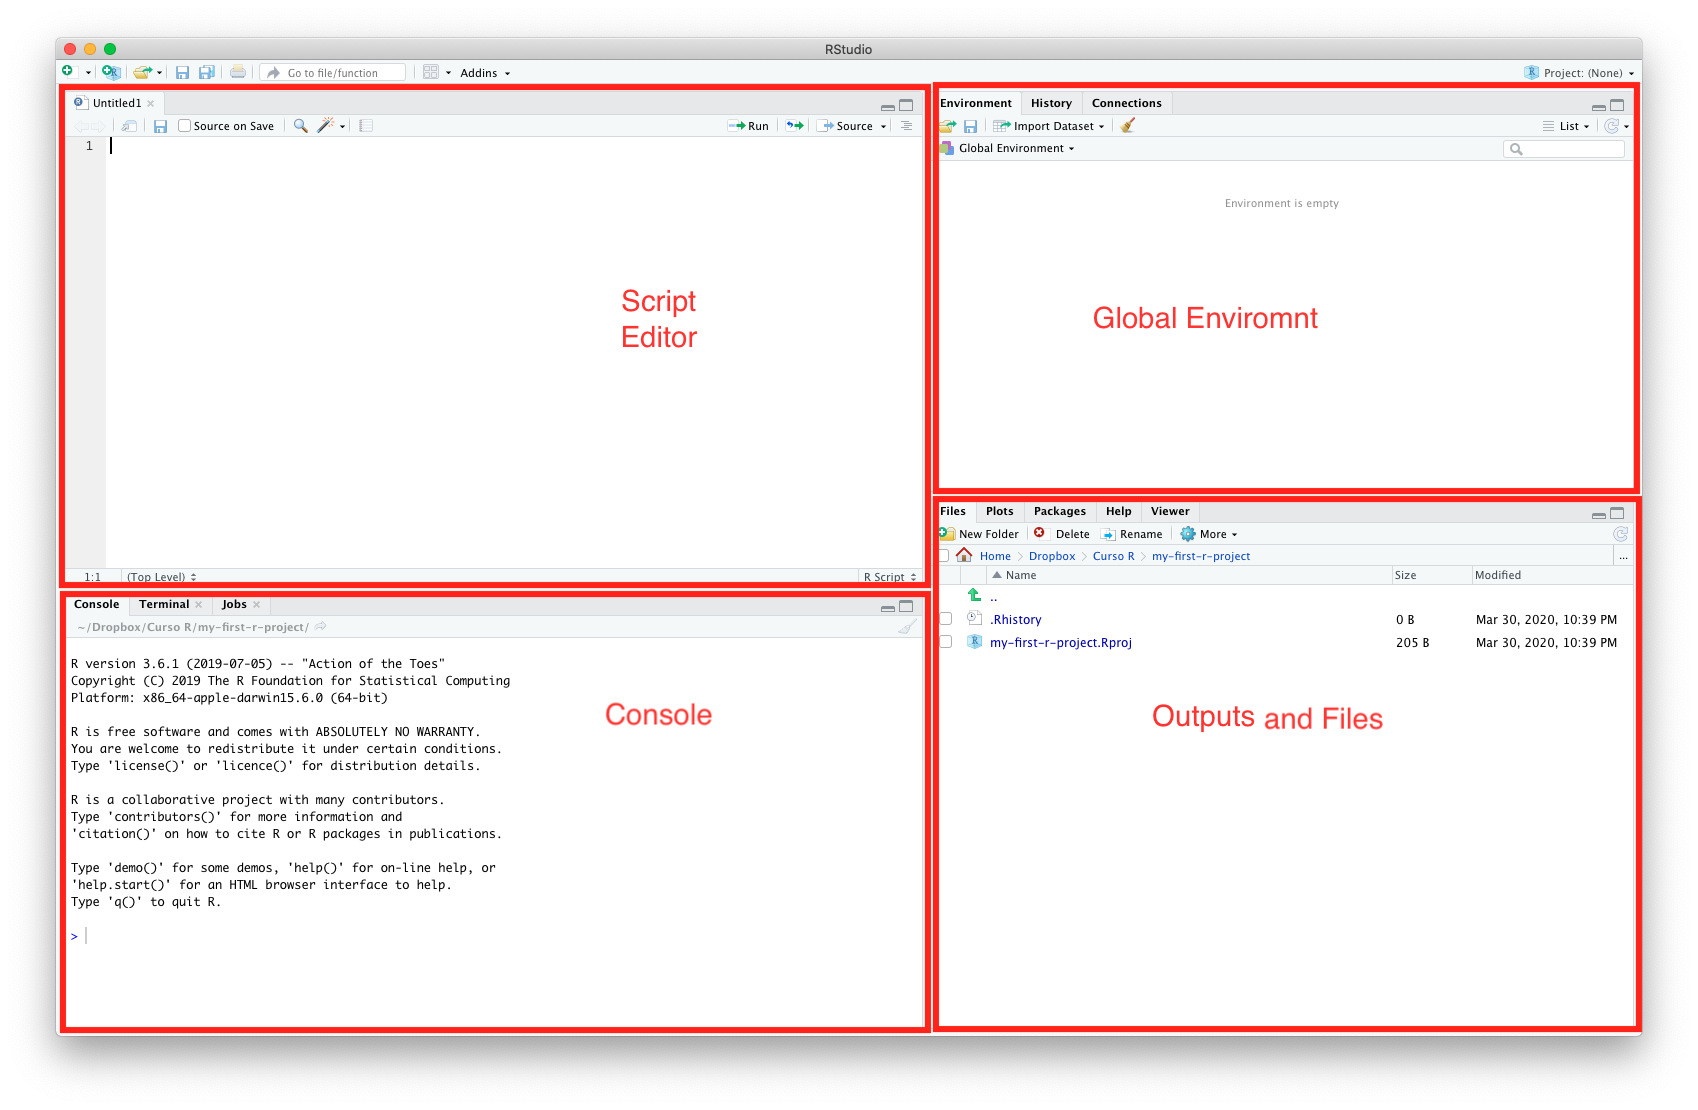
\includegraphics[scale=0.15]{panes.png}
\end{figure}
\end{frame}

\begin{frame}
\frametitle{Editor}
\begin{itemize}
\item The editor is where you can edit the script that you just created. This is where you should write the code that you will learn. 
\item In the editor you can send text to the console, which is where your code will be run.
\item In the editor you can modify, rerun and save your code at any time.
\item If instead you write your code directly in the console, your code will be run but you won't be able to modify it or reuse it later.
\end{itemize}
\end{frame}

\begin{frame}
\frametitle{Some Useful Shortcuts}
\begin{itemize}
\item To save a script use Cmd/Ctrl + S
\item To send code from the editor to the console use cmd/ctrl + enter. This will run the current line of code (or the current selection of lines)
\item To run the whole script use Cmd/Ctrl + Shift + S
\end{itemize}
\end{frame}

\begin{frame}
\frametitle{Example}
\begin{figure}
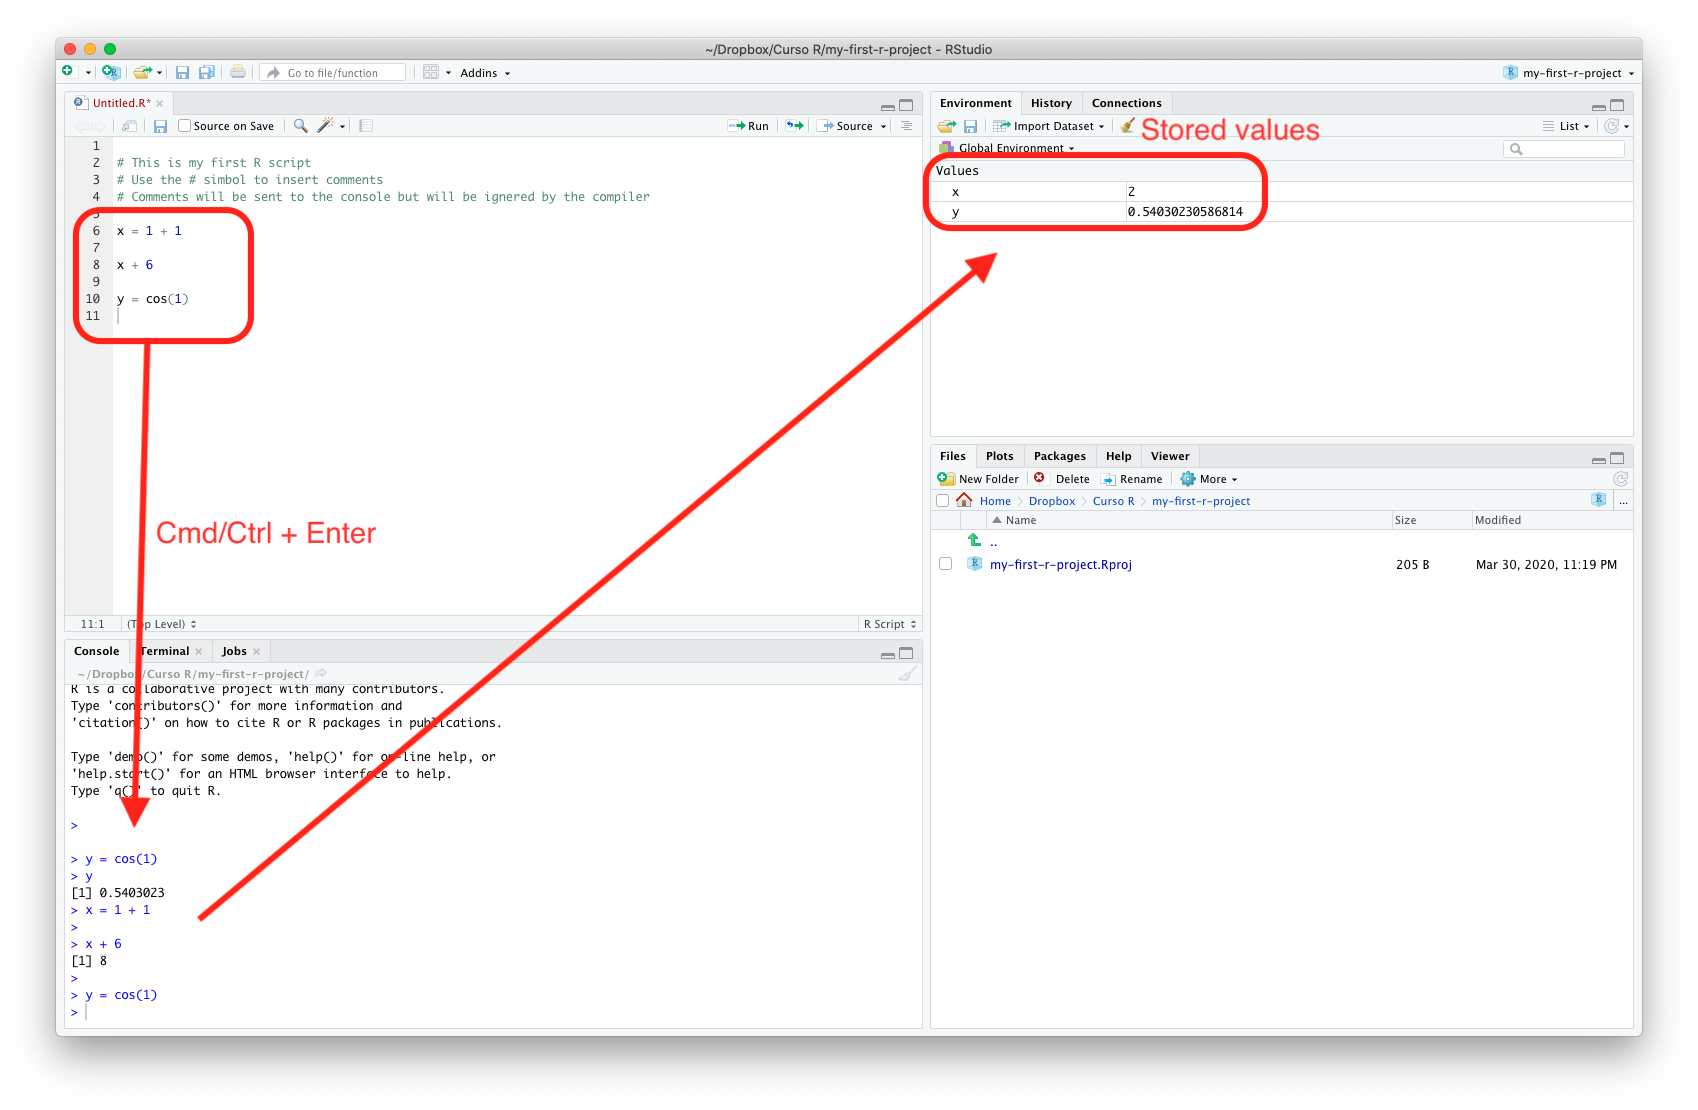
\includegraphics[scale=0.17]{edit-script.png}
\end{figure}
\end{frame}

\begin{frame}
\frametitle{Example (cont.)}
\begin{figure}
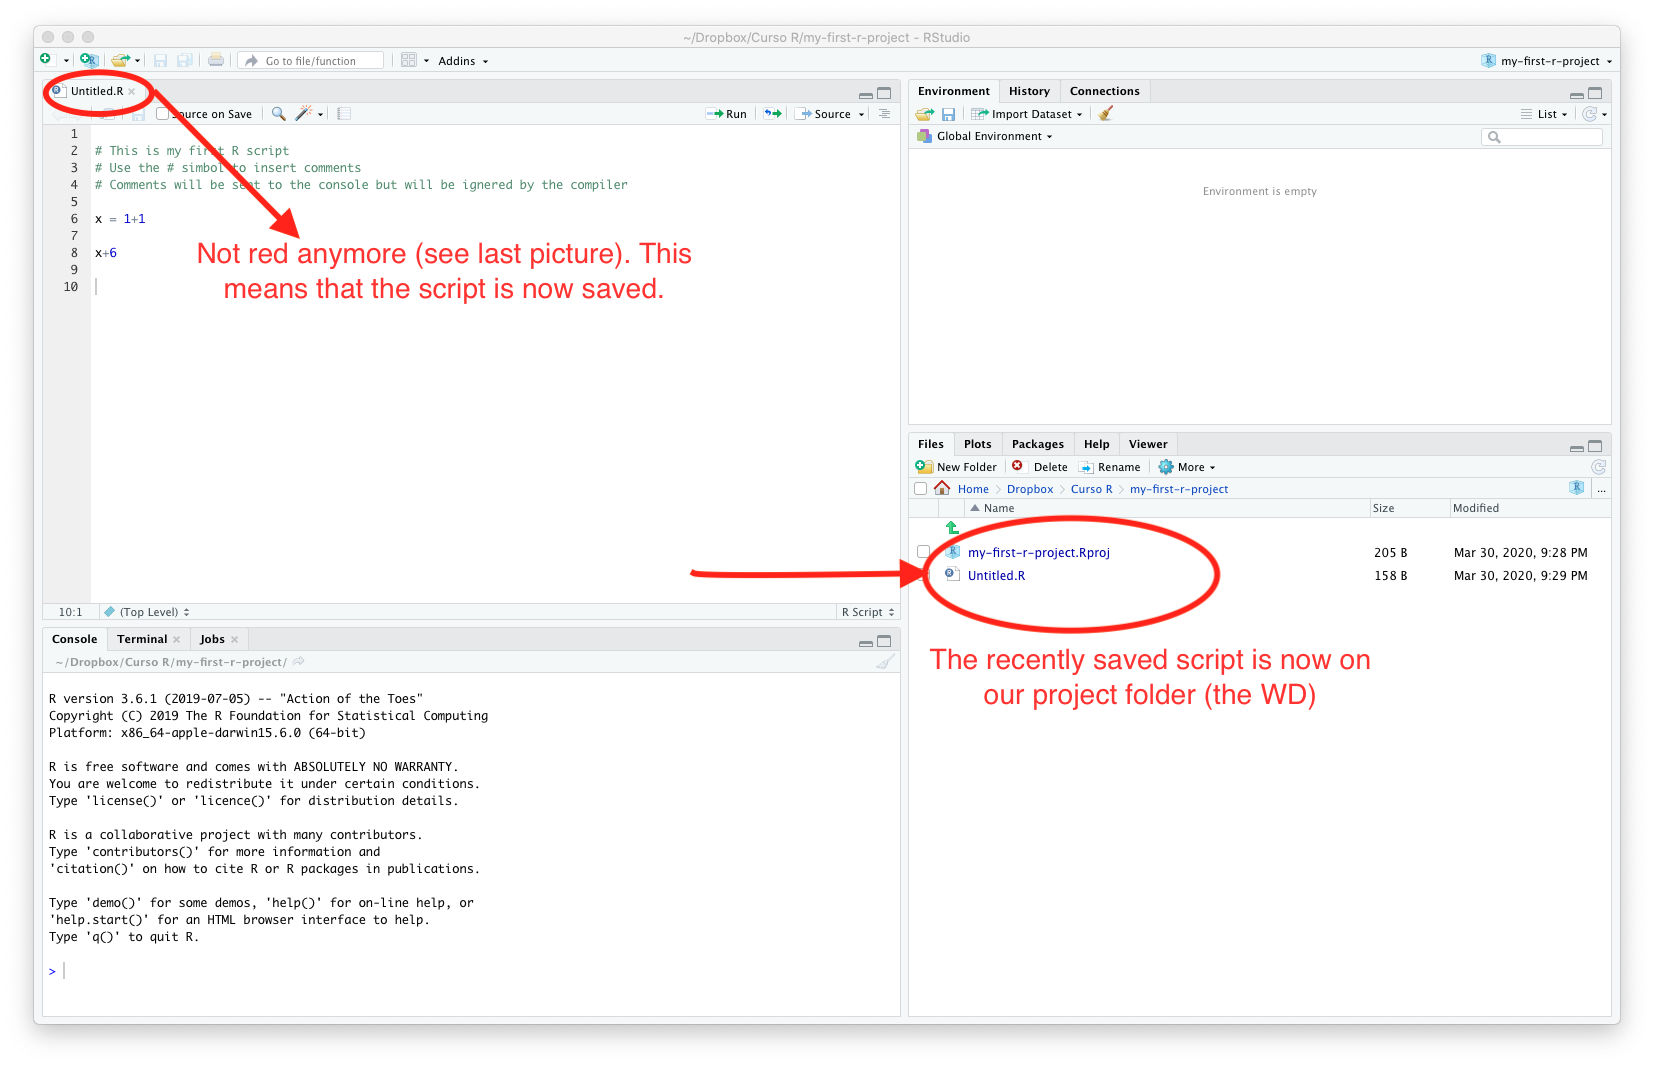
\includegraphics[scale=0.17]{saved-script.png}
\end{figure}
\end{frame}


\subsection{Working Directory}

\begin{frame}[fragile] %%%%%%%%%%%%%%%%%%%%%%% FRAME %%%%%%%%%%%%%%%%%%%%%%%%%%%%
\frametitle{What is a Working Directory?}
\begin{itemize}
\item An active R session always has an associated working directory associated. R will use the working directory by default to:

\begin{itemize}
\item Search for files
\item Save outputs (tables, plots, etc)
\end{itemize}
\end{itemize}

\end{frame}

\begin{frame}
\frametitle{Setting the Working Directory}

\begin{figure}%
   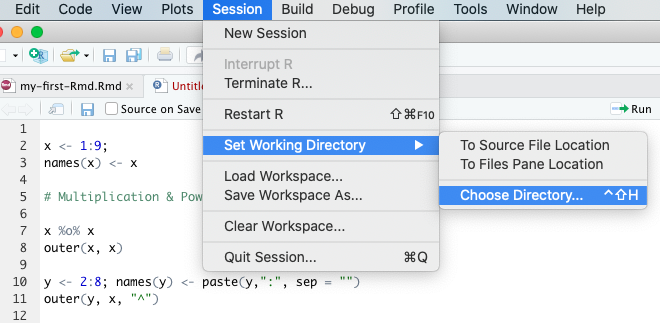
\includegraphics[scale = .38]{wd}
   \caption{Setting the working directory}
\end{figure}

\end{frame}

\begin{frame}[fragile] %%%%%%%%%%%%%%%%%%%%%%% FRAME %%%%%%%%%%%%%%%%%%%%%%%%%%%%
\frametitle{Setting the Working Directory}
\begin{itemize}
\item You can also get or set the working directory in R's console:

\begin{itemize}
\item Getting the working directory
\begin{verbatim}
> getwd()
\end{verbatim}

\item Changing the working directory
\begin{verbatim}
> setwd("/folder1/folder2/folder3/")
\end{verbatim}

\begin{itemize}

\item The problem with commands like this is that such paths will only exist on your computer
\item Solution: Rstudio projects

\end{itemize}
\end{itemize}
\end{itemize}

\end{frame}


\begin{frame}[fragile] %%%%%%%%%%%%%%%%%%%%%%% FRAME %%%%%%%%%%%%%%%%%%%%%%%%%%%%
\frametitle{Advantages of Rstudio Projects}

\begin{itemize}

\item Rstudio projects are self-contained.
\item They put together all the files that are relevant for a particular project (article, book, research project) in the same folder.
\item The project's working directory always points to that folder by default
\item Rstudio projects can be moved around on your computer or onto other computers and will still “\textit{just work}”. No directory changes are needed.
\item If you need to create additional folders or start moving around parts of you project around dont use the \textit{setwd} function. It is safer to reference the full path.

% {\item Search for the package \textit{here}. You can find good references \href{https://malco.io/2018/11/05/why-should-i-use-the-here-package-when-i-m-already-using-projects/}{\textcolor{blue}{here}} and \href{https://github.com/jennybc/here_here}{\textcolor{blue}{here}}}
\end{itemize}


\end{frame}


\section{Packages}

\begin{frame}[fragile] %%%%%%%%%%%%%%%%%%%%%%% FRAME %%%%%%%%%%%%%%%%%%%%%%%%%%%%

\frametitle{Packages}

\begin{itemize}

{\item The more specialized functions and data sets are available on packages (also referred to as libraries).}
\begin{itemize}
\item Installing R Packages:
\begin{verbatim}
> install.packages("ggplot2", dependencies = TRUE)
\end{verbatim}
\item Loading R Packages:
\begin{verbatim}
> library("ggplot2")
\end{verbatim}

\item Updating R Packages:
\begin{verbatim}
> update.packages()  # This is rarely necessary 
\end{verbatim}
\end{itemize}

\item Packages are developed by the R core team and also by the community of R users.

\item You can develop your own packages and make them available to the community on \href{https://cran.r-project.org}{\textcolor{blue}{CRAN}} (The Comprehensive R Archive Network)

\end{itemize}

\end{frame}

\begin{frame}

\frametitle{Packages}

\begin{itemize}
\item It is typically recommend to start your scripts with the packages that you need. 
\item That way, if you share your code with others, they can easily see what packages they need to install. 
\item Note, however, that you should never include \textit{install.packages} or \textit{setwd} in a script that you share. 
\item It is very antisocial to change settings on someone else’s computer!
\end{itemize}

\end{frame}

\section{Settings}

\begin{frame}
\frametitle{Settings and Appearance}
\begin{itemize}
\item You can change Rstudio's default settings and appearence:

\begin{itemize}
\item Mac: Tools $->$ Global Option
\item Windows and Linux: Rstudio $->$ preferences
\end{itemize}

\item Shortcut:
\begin{itemize}
\item Mac: "Cmd" + "," 
\item Windows and Linux: "Ctrl" + "," 
\end{itemize}
\end{itemize}

\end{frame}

\begin{frame}
\frametitle{Settings and Appearance}

\begin{figure}
   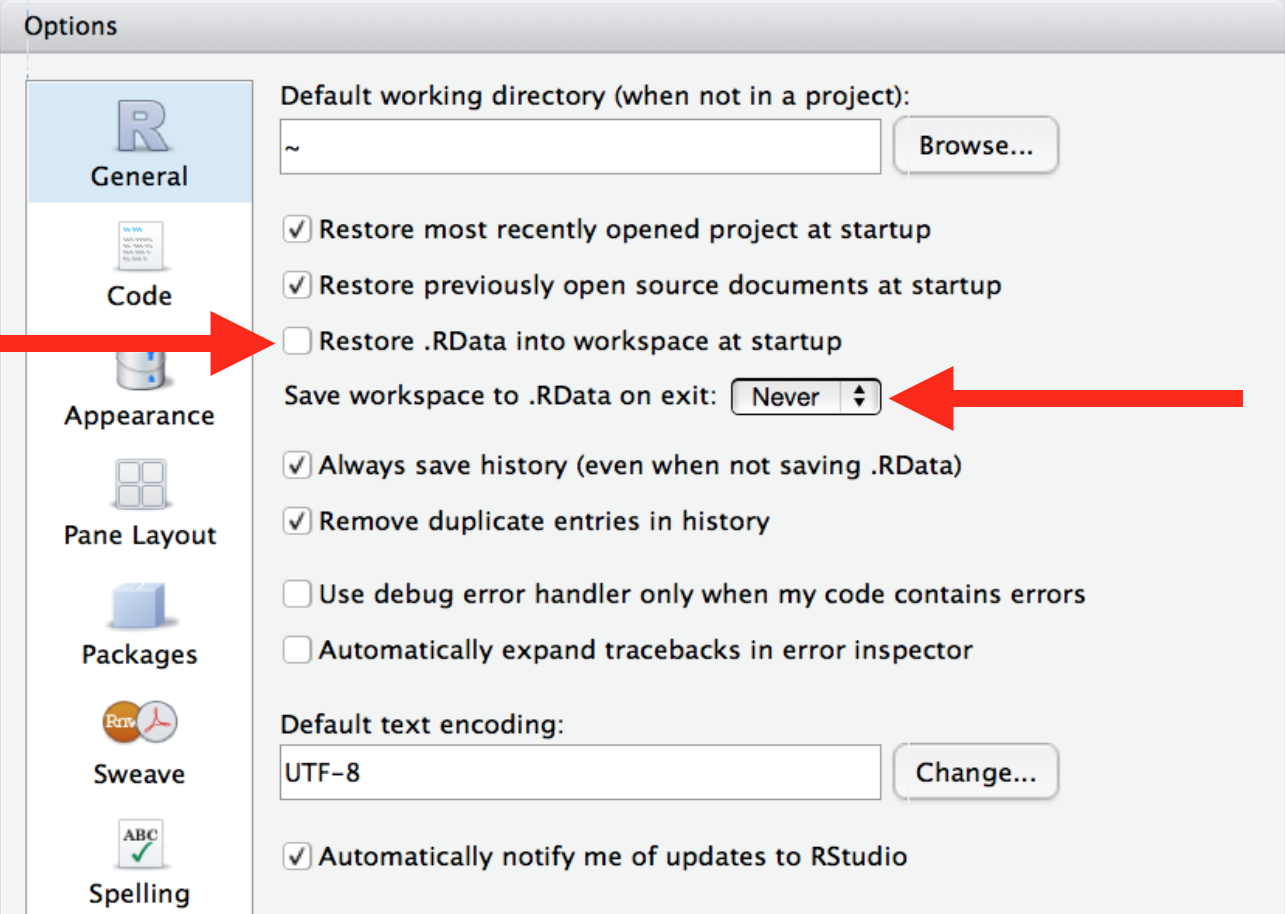
\includegraphics[scale = .3]{settings.png}
   \caption{These are the general settings that we recommend}
\end{figure}
\end{frame}

\begin{frame}[fragile] %%%%%%%%%%%%%%%%%%%%%%% FRAME %%%%%%%%%%%%%%%%%%%%%%%%%%%%
\frametitle{Settings and Appearance}

\begin{figure}%
   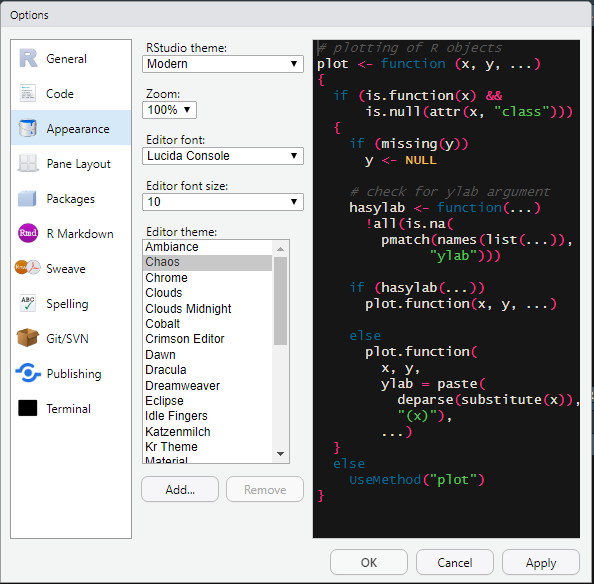
\includegraphics[scale = .35]{Screenshot_4}
   \caption{Changing Rstudio's appearence}
\end{figure}

\end{frame}

\section*{}

\begin{frame} %%%%%%%%%%%%%%%%%%%%%%% FRAME %%%%%%%%%%%%%%%%%%%%%%%%%%%%
\frametitle{Questions?}


\end{frame}
\end{document}

